\documentclass[12pt]{article}
\usepackage[margin=1in]{geometry}
\usepackage{graphicx}
\usepackage{amsmath}
\usepackage{tikz}
\usepackage{hyperref}
\usepackage{enumitem}

\newcommand{\fromlectures}{{\\ \color{blue} \hspace*{\fill}(from lecture slides)} \\}
\newcommand{\bydefn}{{\\ \color{blue} \hspace*{\fill}(by definition)} \\}
\newcommand{\given}{{\\ \color{blue} \hspace*{\fill}(given)} \\}
\newcommand{\rtp}{{\\ \color{blue} \hspace*{\fill}(required to prove)} \\}

\newcommand{\f}[1]{o_{#1}x_{#1}y_{#1}z_{#1}}
\newcommand{\rx}[1]{\begin{bmatrix} 1 & 0 & 0 & 0 \\ 0 & cos(#1) & -sin(#1) & 0 \\ 0 & sin(#1) & cos(#1) & 0 \\ 0 & 0 & 0 & 1 \end{bmatrix}}
\newcommand{\rz}[1]{\begin{bmatrix} cos(#1) & -sin(#1) & 0 & 0 \\ sin(#1) & cos(#1) & 0 & 0 \\ 0 & 0 & 1 & 0 \\ 0 & 0 & 0 & 1 \end{bmatrix}}
\newcommand{\iden}{\begin{bmatrix} 1 & 0 & 0 & 0 \\ 0 & 1 & 0 & 0 \\ 0 & 0 & 1 & 0 \\ 0 & 0 & 0 & 1 \end{bmatrix}}
\newcommand{\trans}[3]{\begin{bmatrix} 1 & 0 & 0 & #1 \\ 0 & 1 & 0 & #2 \\ 0 & 0 & 1 & #3 \\ 0 & 0 & 0 & 1 \end{bmatrix}}

\title{CSci 5551 - HW3}
\author{Yashasvi Sriram Patkuri\\patku001@umn.edu}

\begin{document}
\maketitle
\pagebreak

\section{}
Robot arm has 3 DOF as illustrated in the Figure \ref{fig:q1.1}.
I am assuming that length of link 3 is $L_3$ since it is not mentioned in the figure.
\given

\begin{figure}[h]
  \centering
  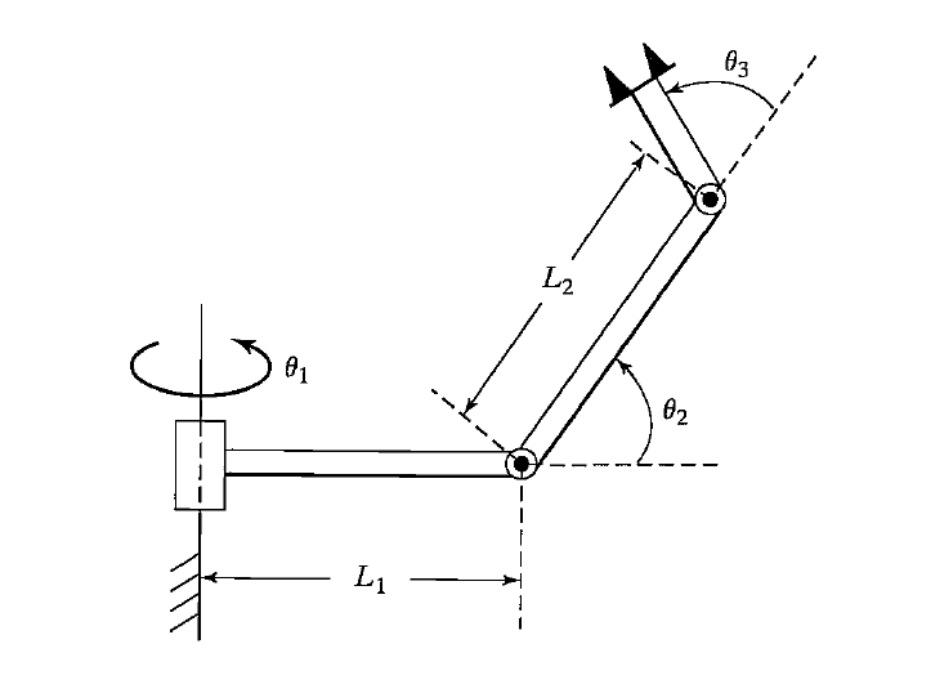
\includegraphics[width=0.6\textwidth]{q1.png}
  \caption{3DOF robot arm}
  \label{fig:q1.1}
\end{figure}

Assigning frames according to DH convention we have,
\fromlectures
\begin{figure}[h]
  \centering
  \begin{tikzpicture}[x=1cm, y=1cm, z=-0.6cm]
    % F1
    \draw [->]       (0, 0) -- (2, 0) node [right] {$x_1$};
    \draw [->]       (0, 0) -- (0, 2) node [left] {$z_1$};
    % F2
    \draw [->]       (4, 0) -- (6, 0) node [right] {$x_2$};
    \draw            (4, 0) circle (0.15cm);
    \draw [fill]     (4, 0) circle (0.07cm) node [left] {$z_2$};
    % F3
    \draw [->]       (6, 2) -- (7.414, 3.414) node [right] {$x_3$};
    \draw            (6, 2) circle (0.15cm);
    \draw [fill]     (6, 2) circle (0.07cm) node [left] {$z_3$};
    % F4
    \draw [->]       (5, 4) -- (3.656, 5.514) node [right] {$x_4$};
    \draw            (5, 4) circle (0.15cm);
    \draw [fill]     (5, 4) circle (0.07cm) node [right] {$z_4$};
  \end{tikzpicture}
  \caption{DH frame assignment}
  \label{fig:q1.2}
\end{figure}
\begin{enumerate}[nolistsep]
  \item The z-axes are chosen along the axes of rotation.
  \item The choice of $z_4$ is free, so it is chosen to be parallel to $z_3$ for simplicity.
  \item The choice of $x_1$ is free, so it chosen in the direction of $x_2$ for simplicity.
  \item $x_2$ lies along the common normal to $z_1$ and $z_2$ which is unique.
  \item There are many common normal to $z_2$ and $z_3$ as they are parallel, so $x_3$ is chosen to be in the plane of paper for simplicity.
  \item $x_4$ is chosen in a similar manner.
  \item Each y-axis (not shown) just form a right handed coordinate system with respective frame.
\end{enumerate}

\subsubsection*{DH parameters}
The DH parameters for the frames shown in Figure \ref{fig:q1.2} are as follows
\begin{center}
\begin{tabular}{ c | c c c c }
 \hline
 $F_i \to F_j$ & $\theta$ & d & r & $\alpha$ \\
 \hline
 $1 \to 2$ & $\theta_1$ & 0 & $L_1$ & $90^{\circ}$ \\
 $2 \to 3$ & $\theta_2$ & 0 & $L_2$ & $0^{\circ}$ \\
 $3 \to 4$ & $\theta_3$ & 0 & $L_3$ & $0^{\circ}$ \\
 \hline
\end{tabular}
\end{center}

\subsubsection*{Transformation from $F_1$ to $F_3$}
\[
  T_{13} \equiv T_{12} * T_{23}
\]
$T_{12}, T_{23}$ can be constructed using DH parameters.
Given frame i and frame j with DH parameters [ $\theta$, d, r, $\alpha$ ] the transformation matrix is
\[
  T_{i,j} \equiv Rot_{z,\theta} * Trans_{z, d} * Trans_{x, r} * Rot_{x, \alpha}
\]
\fromlectures
Consider $T_{12}$
\[
  T_{12} \equiv Rot_{z,\theta_1} * Trans_{z, 0} * Trans_{x, L_1} * Rot_{x, 90^{\circ}}
\]
\[
  T_{12} \equiv \rz{\theta_1} * \trans{0}{0}{0} * \trans{L_1}{0}{0} * \rx{90^{\circ}}
\]
\[
  T_{12} \equiv \rz{\theta_1} * \trans{L_1}{0}{0}
    * \begin{bmatrix} 1 & 0 & 0 & 0 \\ 0 & 0 & -1 & 0 \\ 0 & 1 & 0 & 0 \\ 0 & 0 & 0 & 1 \end{bmatrix}
\]
\[
  T_{12} \equiv \rz{\theta_1}
  * \begin{bmatrix} 1 & 0 & 0 & L_1 \\ 0 & 0 & -1 & 0 \\ 0 & 1 & 0 & 0 \\ 0 & 0 & 0 & 1 \end{bmatrix}
\]
\[
  T_{12} \equiv
  \begin{bmatrix} c\theta_1 & 0 & s\theta_1 & L_1c\theta_1 \\ s\theta_1 & 0 & -c\theta_1 & L_1s\theta_1 \\ 0 & 1 & 0 & 0 \\ 0 & 0 & 0 & 1 \end{bmatrix}
\]

Consider $T_{23}$
\[
  T_{23} \equiv Rot_{z,\theta_2} * Trans_{z, 0} * Trans_{x, L_2} * Rot_{x, 0^{\circ}}
\]
\[
  T_{23} \equiv \rz{\theta_2} * \trans{0}{0}{0} * \trans{L_2}{0}{0} * \rx{0^{\circ}}
\]
\[
  T_{23} \equiv \rz{\theta_2} * \trans{0}{0}{0} * \trans{L_2}{0}{0} * \iden
\]
\[
  T_{23} \equiv \rz{\theta_2} * \trans{L_2}{0}{0}
\]
\[
  T_{23} \equiv
  \begin{bmatrix} c\theta_2 & -s\theta_2 & 0 & L_2c\theta_2 \\ s\theta_2 & c\theta_2 & 0 & L_2s\theta_2 \\ 0 & 0 & 1 & 0 \\ 0 & 0 & 0 & 1 \end{bmatrix}
\]

\[
  T_{13} \equiv T_{12} * T_{23}
\]
Substituting $T_{12}, T_{23}$ we have,
\[
  T_{13} \equiv
  \begin{bmatrix} c\theta_1 & 0 & s\theta_1 & L_1c\theta_1 \\ s\theta_1 & 0 & -c\theta_1 & L_1s\theta_1 \\ 0 & 1 & 0 & 0 \\ 0 & 0 & 0 & 1 \end{bmatrix}
  *
  \begin{bmatrix} c\theta_2 & -s\theta_2 & 0 & L_2c\theta_2 \\ s\theta_2 & c\theta_2 & 0 & L_2s\theta_2 \\ 0 & 0 & 1 & 0 \\ 0 & 0 & 0 & 1 \end{bmatrix}
\]
\[
  T_{13} \equiv
  \begin{bmatrix}
    c\theta_1c\theta_2 & -c\theta_1s\theta_2 & s\theta_1 & L_2c\theta_1c\theta_2 + L_1c\theta_1 \\
    s\theta_1c\theta_2 & -s\theta_1s\theta_2 & -c\theta_1 & L_2s\theta_1c\theta_2 + L_1s\theta_1 \\
    s\theta_2 & c\theta_2 & 0 & L_2s\theta_2 \\
    0 & 0 & 0 & 1
  \end{bmatrix}
\]

\pagebreak

\section{}
Robot arm has 6 DOF as illustrated in the Figure \ref{fig:q2.1}.
\given

\begin{figure}[h]
  \centering
  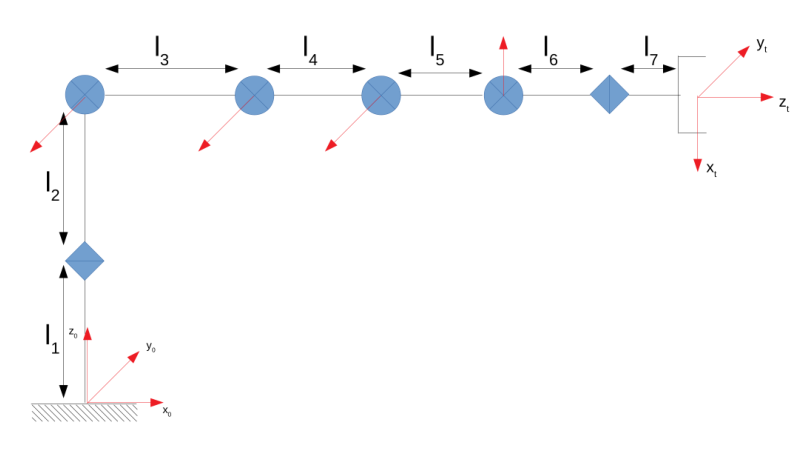
\includegraphics[width=0.6\textwidth]{q2.png}
  \caption{6DOF robot arm}
  \label{fig:q2.1}
\end{figure}

Assigning frames according to DH convention we have,
\fromlectures
\begin{figure}[h]
  \centering
  \begin{tikzpicture}[x=1cm, y=1cm, z=-0.6cm]
    % F0
    \draw [->]       (0, 0) -- (1, 0) node [right] {$x_0$};
    \draw [->]       (0, 0) -- (0, 1) node [left] {$z_0$};
    % F1
    \draw [->]       (0, 2) -- (1, 2) node [right] {$x_1$};
    \draw [->]       (0, 2) -- (0, 3) node [left] {$z_1$};
    % F2
    \draw [->]       (0, 4) -- (1, 4) node [right] {$x_2$};
    \draw            (0, 4) circle (0.15cm);
    \draw [fill]     (0, 4) circle (0.07cm) node [left] {$z_2$};
    % F3
    \draw [->]       (3, 4) -- (4, 4) node [right] {$x_3$};
    \draw            (3, 4) circle (0.15cm);
    \draw [fill]     (3, 4) circle (0.07cm) node [left] {$z_3$};
    % F4
    \draw [->]       (6, 4) -- (7, 4) node [right] {$x_4$};
    \draw            (6, 4) circle (0.15cm);
    \draw [fill]     (6, 4) circle (0.07cm) node [left] {$z_4$};
    % F5
    \draw [->]       (9, 4) -- (10, 4) node [right] {$x_5, z_6$};
    \draw [->]       (9, 4) -- (9, 5) node [left] {$z_5$};
    \draw            (9, 4) circle (0.15cm);
    \draw [fill]     (9, 4) circle (0.07cm) node [left] {$x_6$};
    % F6
    \draw [->]       (15, 4) -- (16, 4) node [right] {$z_t$};
    \draw [->]       (15, 4) -- (15, 3) node [left] {$x_t$};
  \end{tikzpicture}
  \caption{DH frame assignment}
  \label{fig:q2.2}
\end{figure}
\begin{enumerate}[nolistsep]
  \item The z-axes are chosen along the axes of rotation or translation.
  \item $z_0$, $z_1$ are co-incident, therefore $x_1$ is chosen at the end of link 1 for simplicity.
  \item $z_1$, $z_2$ intersection is taken as origin of $F_2$ with $x_2$ perpendicular to plane formed by $z_2$ and $z_1$.
  \item $z_2$, $z_3$ are parallel so $x_3$ is chosen to be on plane of paper for simplicity.
  \item $x_4$ is chosen in the same ways as $x_3$.
  \item $z_4$, $z_5$ have a unique common normal, thus there is only one choice of $x_5$.
  \item $z_5$, $z_6$ intersection is taken as origin of $F_6$ with $x_6$ perpendicular to plane formed by $z_5$ and $z_6$.
  \item Note that this step is probably most non-trivial in this procedure as origins of $F_5$ and $F_6$ coincide.
\end{enumerate}

\subsubsection*{DH parameters}
I am assuming that the lengths $l_2$ and $l_7$ are constant link lengths and the prismatic joints $J_1$ and $J_6$ provide additional (signed) lengths of $q_1$ and $q_6$ respectively.
With this the DH parameters for the frames shown in Figure \ref{fig:q2.2} are as follows,
\begin{center}
\begin{tabular}{ c | c c c c }
 \hline
 $F_i \to F_j$ & $\theta$ & d & r & $\alpha$ \\
 \hline
 $0 \to 1$ & $0^{\circ}$    & $l_1$                      & $0$     &   $0^{\circ}$   \\
 $1 \to 2$ & $0^{\circ}$    & $l_2 + q_1$                & $0$     &   $90^{\circ}$  \\
 $2 \to 3$ & $q_2$          & $0$                        & $l_3$   &   $0^{\circ}$   \\
 $3 \to 4$ & $q_3$          & $0$                        & $l_4$   &   $0^{\circ}$   \\
 $4 \to 5$ & $q_4$          & $0$                        & $l_5$   &   $-90^{\circ}$ \\
 $5 \to 6$ & $q_5$          & $0$                        & $0$     &   $-90^{\circ}$ \\
 $6 \to t$ & $90^{\circ}$   & $l_6 + l_7 + q_6$          & $0$     &   $0^{\circ}$ \\
 \hline
\end{tabular}
\end{center}

\subsubsection*{Transformation from $F_0$ to $F_4$}
\[
  T_{04} \equiv T_{01} * T_{12} * T_{23} * T_{34}
\]
$T_{01}, T_{12}, T_{23}, T_{34}$ can be constructed using DH parameters.
Given frame i and frame j with DH parameters [ $\theta$, d, r, $\alpha$ ] the transformation matrix is
\[
  T_{i,j} \equiv Rot_{z,\theta} * Trans_{z, d} * Trans_{x, r} * Rot_{x, \alpha}
\]
\fromlectures
Consider $T_{01}$,
\[
  T_{01} \equiv Rot_{z, 0} * Trans_{z, l_1} * Trans_{x, 0} * Rot_{x, 0^{\circ}}
\]
\[
  T_{01} \equiv \rz{0} * \trans{0}{0}{l_1} * \trans{0}{0}{0} * \rx{0^{\circ}}
\]
Evaluating trigs,
\[
  T_{01} \equiv \iden * \trans{0}{0}{l_1} * \trans{0}{0}{0} * \iden
\]
Removing identities,
\[
  T_{01} \equiv \trans{0}{0}{l_1}
\]
Consider $T_{12}$,
\[
  T_{12} \equiv Rot_{z, 0} * Trans_{z, l_2 + q_1} * Trans_{x, 0} * Rot_{x, 90^{\circ}}
\]
\[
  T_{12} \equiv \rz{0} * \trans{0}{0}{l_2 + q_1} * \trans{0}{0}{0} * \rx{90^{\circ}}
\]
Evaluating trigs,
\[
  T_{12} \equiv \iden * \trans{0}{0}{l_2 + q_1} * \trans{0}{0}{0}
  * \begin{bmatrix} 1 & 0 & 0 & 0 \\ 0 & 0 & -1 & 0 \\ 0 & 1 & 0 & 0 \\ 0 & 0 & 0 & 1 \end{bmatrix}
\]
Removing identities,
\[
  T_{12} \equiv \trans{0}{0}{l_2 + q_1}
  * \begin{bmatrix} 1 & 0 & 0 & 0 \\ 0 & 0 & -1 & 0 \\ 0 & 1 & 0 & 0 \\ 0 & 0 & 0 & 1 \end{bmatrix}
\]
\[
  T_{12} \equiv
  \begin{bmatrix} 1 & 0 & 0 & 0 \\ 0 & 0 & -1 & 0 \\ 0 & 1 & 0 & l_2 + q_1 \\ 0 & 0 & 0 & 1 \end{bmatrix}
\]
Consider $T_{23}$,
\[
  T_{23} \equiv Rot_{z, q_2} * Trans_{z, 0} * Trans_{x, l_3} * Rot_{x, 0^{\circ}}
\]
\[
  T_{23} \equiv \rz{q_2} * \trans{0}{0}{0} * \trans{l_3}{0}{0} * \rx{0^{\circ}}
\]
Evaluating trigs,
\[
  T_{23} \equiv \rz{q_2} * \trans{0}{0}{0} * \trans{l_3}{0}{0} * \iden
\]
Removing identities,
\[
  T_{23} \equiv \rz{q_2} * \trans{l_3}{0}{0}
\]
\[
  T_{23} \equiv
  \begin{bmatrix} cq_2 & -sq_2 & 0 & l_3cq_2 \\ sq_2 & cq_2 & 0 & l_3sq_2 \\ 0 & 0 & 1 & 0 \\ 0 & 0 & 0 & 1 \end{bmatrix}
\]
Consider $T_{34}$,
\[
  T_{34} \equiv Rot_{z, q_3} * Trans_{z, 0} * Trans_{x, l_4} * Rot_{x, 0^{\circ}}
\]
This is same as $T_{23}$ except for the variables, therefore we can use the final form of $T_{23}$ with replaced variables.
\[
  T_{34} \equiv
  \begin{bmatrix} cq_3 & -sq_3 & 0 & l_4cq_3 \\ sq_3 & cq_3 & 0 & l_4sq_3 \\ 0 & 0 & 1 & 0 \\ 0 & 0 & 0 & 1 \end{bmatrix}
\]
Finally,
\[
  T_{04} \equiv T_{01} * T_{12} * T_{23} * T_{34}
\]
\[
  T_{04} \equiv
  \trans{0}{0}{l_1}
  *
  \begin{bmatrix} 1 & 0 & 0 & 0 \\ 0 & 0 & -1 & 0 \\ 0 & 1 & 0 & l_2 + q_1 \\ 0 & 0 & 0 & 1 \end{bmatrix}
  *
  \begin{bmatrix} cq_2 & -sq_2 & 0 & l_3cq_2 \\ sq_2 & cq_2 & 0 & l_3sq_2 \\ 0 & 0 & 1 & 0 \\ 0 & 0 & 0 & 1 \end{bmatrix}
  *
  \begin{bmatrix} cq_3 & -sq_3 & 0 & l_4cq_3 \\ sq_3 & cq_3 & 0 & l_4sq_3 \\ 0 & 0 & 1 & 0 \\ 0 & 0 & 0 & 1 \end{bmatrix}
\]
Multiplying first two,
\[
  T_{04} \equiv
  \begin{bmatrix} 1 & 0 & 0 & 0 \\ 0 & 0 & -1 & 0 \\ 0 & 1 & 0 & l_1 + l_2 + q_1 \\ 0 & 0 & 0 & 1 \end{bmatrix}
  *
  \begin{bmatrix} cq_2 & -sq_2 & 0 & l_3cq_2 \\ sq_2 & cq_2 & 0 & l_3sq_2 \\ 0 & 0 & 1 & 0 \\ 0 & 0 & 0 & 1 \end{bmatrix}
  *
  \begin{bmatrix} cq_3 & -sq_3 & 0 & l_4cq_3 \\ sq_3 & cq_3 & 0 & l_4sq_3 \\ 0 & 0 & 1 & 0 \\ 0 & 0 & 0 & 1 \end{bmatrix}
\]
Multiplying last two,
\[
  T_{04} \equiv
  \begin{bmatrix} 1 & 0 & 0 & 0 \\ 0 & 0 & -1 & 0 \\ 0 & 1 & 0 & l_1 + l_2 + q_1 \\ 0 & 0 & 0 & 1 \end{bmatrix}
  *
  \begin{bmatrix}
    cq_2cq_3 - sq_2sq_3 & -(sq_2cq_3 + cq_2sq_3) & 0 & l_4(cq_2cq_3 - sq_2sq_3) + l_3cq_2 \\
    sq_2cq_3 + cq_2sq_3 & cq_2cq_3 - sq_2sq_3    & 0 & l_4(sq_2cq_3 + cq_2sq_3) + l_3sq_2 \\
    0                   & 0                      & 1 & 0 \\
    0                   & 0                      & 0 & 1
  \end{bmatrix}
\]
Using trig identity $s(a + b) \equiv s(a)c(b) + c(a)s(b), c(a + b) \equiv c(a)c(b) - s(a)s(b)$
\[
  T_{04} \equiv
  \begin{bmatrix} 1 & 0 & 0 & 0 \\ 0 & 0 & -1 & 0 \\ 0 & 1 & 0 & l_1 + l_2 + q_1 \\ 0 & 0 & 0 & 1 \end{bmatrix}
  *
  \begin{bmatrix}
    c(q_2 + q_3) & -s(q_2 + q_3) & 0 & l_4c(q_2 + q_3) + l_3cq_2 \\
    s(q_2 + q_3) & c(q_2 + q_3)  & 0 & l_4s(q_2 + q_3) + l_3sq_2 \\
    0            & 0             & 1 & 0 \\
    0            & 0             & 0 & 1
  \end{bmatrix}
\]
\[
  T_{04} \equiv
  \begin{bmatrix}
    c(q_2 + q_3) & -s(q_2 + q_3) & 0 & l_4c(q_2 + q_3) + l_3cq_2 \\
    0 & 0 & -1 & 0 \\
    s(q_2 + q_3) & c(q_2 + q_3)  & 0 & l_4s(q_2 + q_3) + l_3sq_2 + l_1 + l_2 + q_1 \\
    0 & 0 & 0 & 1 \\
  \end{bmatrix}
\]

\pagebreak

\section{}
MOM manipulator is illustrated in the Figure \ref{fig:q3.1}.
The lengths of various parts are labeled on the image in red ink.
Specifically the distance from base to joint 1 is $l_1$, distance b/w shoulder and forearm is $l_2$ and the distance b/w wrist and end-effector is $l_3$.
\given
\begin{figure}[h]
  \centering
  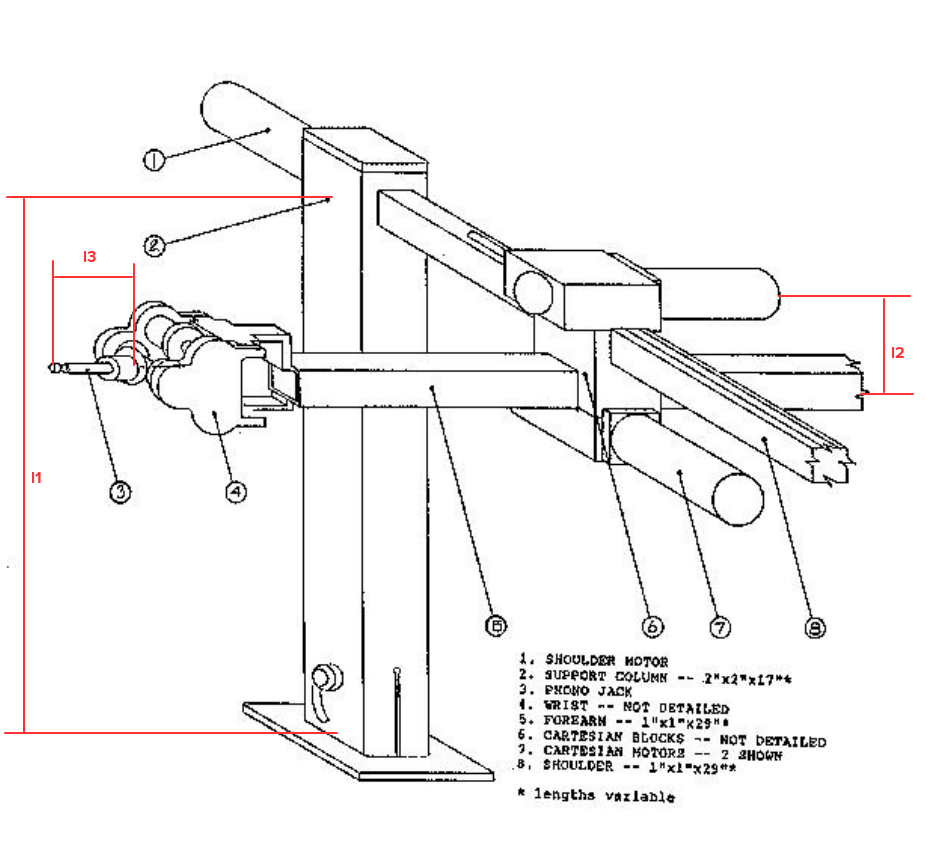
\includegraphics[width=1\textwidth]{q3.png}
  \caption{MOM manipulator}
  \label{fig:q3.1}
\end{figure}

\pagebreak
Assigning frames according to DH convention we have,
\fromlectures
\begin{figure}[h]
  \centering
  \begin{tikzpicture}[x=1cm, y=1cm, z=-0.6cm]
    \draw [dashed, red]       (-2, -3) -- (-2, 2) node [right] {$l_1$};
    \draw [dashed, red]       (5, 2) -- (5, 1) node [right] {$l_2$};
    % F0
    \draw [->]       (0, -3) -- (0, -2) node [right] {$z_0$};
    \draw            (0, -3) circle (0.15cm);
    \draw [fill]     (0, -3) circle (0.07cm) node [right] {$x_0$};
    % F1,2
    \draw [->]       (0, 2) -- (1, 2) node [right] {$z_1, z_2$};
    \draw            (0, 2) circle (0.15cm);
    \draw [fill]     (0, 2) circle (0.07cm) node [left] {$x_1, x_2$};
    % F3
    \draw [->]       (4, 1) -- (4, 0) node [right] {$x_3$};
    \draw            (4, 1) circle (0.15cm);
    \draw [fill]     (4, 1) circle (0.07cm) node [right] {$z_3$};
  \end{tikzpicture}
  \caption{DH frame assignment for joints 1-3: Front view}
  \label{fig:q3.2}
\end{figure}
\begin{figure}[h]
  \centering
  \begin{tikzpicture}[x=1cm, y=1cm, z=-0.6cm]
    \draw [dashed, red]       (3, -2) -- (-1, -2) node [left] {$l_3$};
    % F3
    \draw [->]       (7, 1) -- (7, 0) node [left] {$x_3$};
    \draw [->]       (7, 1) -- (6, 1) node [left] {$z_3$};
    % F4,5,6
    \draw [->]       (3, 1) -- (3, 0) node [left] {$x_4$};
    \draw [->]       (3, 1) -- (3, 2) node [left] {$z_5$};
    \draw [->]       (3, 1) -- (2, 1) node [left] {$z_4, z_6$};
    \draw            (3, 1) circle (0.15cm);
    \draw [fill]     (3, 1) circle (0.07cm) node [right] {$x_5, x_6$};
    % F7
    \draw [->]       (-1, 1) -- (-2, 1) node [left] {$z_7$};
    \draw            (-1, 1) circle (0.15cm);
    \draw [fill]     (-1, 1) circle (0.07cm) node [right] {$x_7$};
  \end{tikzpicture}
  \caption{DH frame assignment for joints 4-7: Side view}
  \label{fig:q3.3}
\end{figure}
\begin{enumerate}[nolistsep]
  \item The base frame z-axis is chosen to be upward and its x-axis in the direction of end-effector for the pose in Figure \ref{fig:q3.1}.
  \item The side in which $x_0$ comes out of paper and $z_0$ goes up is referred to as the front view in Figure \ref{fig:q3.2}. The side view formed by it is used in Figure \ref{fig:q3.3}.
  \item The end-effector frame z-axis is chosen as shown in Figure \ref{fig:q3.3}.
  \item The z-axes are chosen along the axes of rotation/translation.
  \item $z_0$ and $z_1$ intersection is taken as origin of $F_1$, $x_1$ is chosen to be normal to plane formed by $z_0$ and $z_1$.
  \item $z_1$ and $z_2$ coincide, so $x_2$ is chosen to be coincident to $x_1$ for simplicity.
  \item $z_2$ and $z_3$ have a unique common normal, so $x_3$ is chosen according to that.
  \item $F_1 \to F_2$ captures joint 1 effect. $F_2 \to F_3$ captures joint 2 effect.
  \item Spherical joint is made using three rotational joints as described in lecture slides captured by frames $F_4, F_5, F_6$.
  \item $z_3$ and $z_4$ are coincident, so $x_4$ is chosen to be on the end of forearm for simplicity.
  \item $z_4$ and $z_5$ intersection is taken as origin for $F_5$ and $x_5$ is chosen perpendicular to plane of $z_4$ and $z_5$.
  \item $x_6$ is chosen in the same way.
  \item $z_6$ and $z_7$ are coincident so $x_7$ is chosen on the end-effector for simplicity.
  \item Each y-axis (not shown) just form a right handed coordinate system with respective frame.
\end{enumerate}

\subsubsection*{DH parameters}
DH parameters for the frames shown in Figure \ref{fig:q3.2} and \ref{fig:q3.3} are as follows,
\begin{center}
\begin{tabular}{ c | c c c c }
 \hline
 $F_i \to F_j$ & $\theta$ & d & r & $\alpha$ \\
 \hline
 $0 \to 1$ & $0^{\circ}$    & $l_1$                      & $0$     &   $-90^{\circ}$    \\
 $1 \to 2$ & $q_1$          & $0$                        & $0$     &   $0^{\circ}$      \\
 $2 \to 3$ & $90^{\circ}$   & $q_2$                      & $l_2$   &   $90^{\circ}$     \\
 $3 \to 4$ & $0^{\circ}$    & $q_3$                      & $0$     &   $0^{\circ}$      \\
 $4 \to 5$ & $q_4$          & $0$                        & $0$     &   $-90^{\circ}$    \\
 $5 \to 6$ & $q_5$          & $0$                        & $0$     &   $90^{\circ}$     \\
 $6 \to 7$ & $q_6$          & $l_3$                      & $0$     &   $0^{\circ}$      \\
 \hline
\end{tabular}
\end{center}

\pagebreak

\section{}
A human hand is illustrated in the Figure \ref{fig:q4.1}.
The lengths of various parts are labeled on the image in red ink.
Specifically the distance from shoulder joint to elbow is $l_1$, distance from elbow and wrist is $l_2$ and the distance from wrist and tip of fingers is $l_3$.
The joints in the fingers are ignored.
\given
\begin{figure}[h]
  \centering
  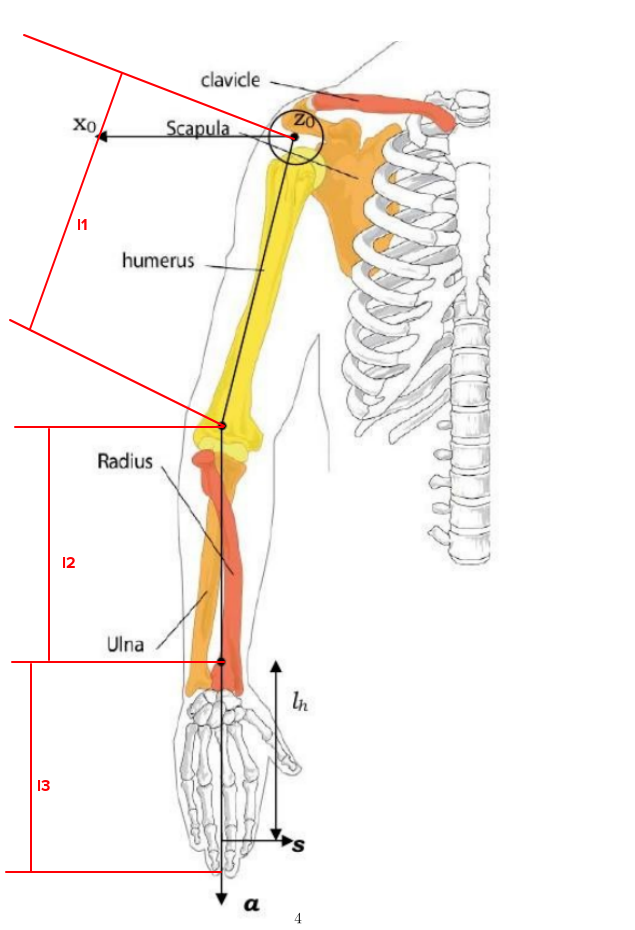
\includegraphics[width=0.68\textwidth]{q4.png}
  \caption{Human hand}
  \label{fig:q4.1}
\end{figure}

\pagebreak
Assigning frames according to DH convention we have,
\fromlectures
\begin{figure}[h]
  \centering
  \begin{tikzpicture}[x=1cm, y=1cm, z=-0.6cm]
    \draw [dashed, red]       (-3, 0) -- (-3, -5) node [right] {$l_1$};
    \draw [dashed, red]       (3, -5) -- (3, -10) node [right] {$l_2$};
    \draw [dashed, red]       (-3, -10) -- (-3, -12) node [right] {$l_3$};
    % F1,2,3
    \draw [->]       (0, 0) -- (-1, 0) node [left] {$x_0, x_1$};
    \draw            (0, 0) circle (0.15cm);
    \draw [fill]     (0, 0) circle (0.07cm) node [below] {$z_0, x_2$};
    \draw [->]       (0, 0) -- (0, 1) node [left] {$z_1$};
    \draw [->]       (0, 0) -- (1, 0) node [right] {$z_2$};
    % F4,5
    \draw [->]       (0, -5) -- (0, -6) node [left] {$x_3, z_4$};
    \draw [->]       (0, -5) -- (1, -5) node [right] {$x_4$};
    \draw            (0, -5) circle (0.15cm);
    \draw [fill]     (0, -5) circle (0.07cm) node [above] {$z_3$};
    % F6,7
    \draw [->]       (0, -10) -- (0, -9) node [left] {$x_6$};
    \draw [->]       (0, -10) -- (1, -10) node [right] {$x_5, z_6$};
    \draw            (0, -10) circle (0.15cm);
    \draw [fill]     (0, -10) circle (0.07cm) node [below] {$z_5$};
    % F8
    \draw [->]       (0, -12) -- (0, -11) node [left] {$x_7$};
    \draw [->]       (0, -12) -- (1, -12) node [right] {$z_7$};
  \end{tikzpicture}
  \caption{DH frame assignment}
  \label{fig:q4.2}
\end{figure}
\begin{enumerate}[nolistsep]
  \item The spherical joint at the shoulder is modeled using 3 revolute joints captured by $F_0, F_1, F_2$, elbow by $F_3$ and wrist by $F_4, F_5, F_6$ and tip of hand by $F_7$. The lengths labeled in Figure \ref{fig:q4.1} are replicated in Figure \ref{fig:q4.2}.
    \begin{enumerate}[nolistsep]
      \item $F_0$ models sideways rotation.
      \item $F_1$ models hand twisting rotation.
      \item $F_2$ models forward/backward rotation.
      \item $F_3$ models elbow rotation
      \item $F_4$ models forearm axial roll.
      \item $F_5$ models wrist yaw.
      \item $F_6$ models wrist pitch.
    \end{enumerate}
  \item z-axes are chosen using joints.
  \item $z_0, z_1$ intersection point is chosen as origin for $F_1$, and $x_1$ is chosen perpendicular to $z_0, z_1$.
  \item $x_2$ is chosen similarly.
  \item $z_2, z_3$ have a unique common normal, so $x_3$ is chosen along that.
  \item $z_3, z_4$ intersection point is chosen as origin for $F_4$, and $x_4$ is chosen perpendicular to $z_3, z_4$.
  \item $x_5, x_6$ are chosen similarly.
  \item $F_7$ is chosen with same orientation as $F_6$ but translated to tip of hand for simplicity.
\end{enumerate}

\subsubsection*{DH parameters}
DH parameters for the frames shown in Figure \ref{fig:q4.2} are as follows,
\begin{center}
\begin{tabular}{ c | c c c c }
 \hline
 $F_i \to F_j$ & $\theta$ & d & r & $\alpha$ \\
 \hline
 $0 \to 1$ & $q_1$    & $0$       & $0$     &   $90^{\circ}$   \\
 $1 \to 2$ & $q_2$    & $0$       & $0$     &   $-90^{\circ}$  \\
 $2 \to 3$ & $q_3$    & $0$       & $l_1$   &   $90^{\circ}$   \\
 $3 \to 4$ & $q_4$    & $0$       & $0$     &   $90^{\circ}$   \\
 $4 \to 5$ & $q_5$    & $l_2$     & $0$     &   $-90^{\circ}$  \\
 $5 \to 6$ & $q_6$    & $0$       & $0$     &   $90^{\circ}$   \\
 $6 \to 7$ & $q_7$    & $0$       & $-l_3$  &   $0^{\circ}$    \\
 \hline
\end{tabular}
\end{center}

\end{document}
